\documentclass[10pt,a4paper]{article}
\usepackage[utf8]{inputenc}
\usepackage[T1]{fontenc}
\usepackage[margin=0.5in]{geometry}
\usepackage{xcolor}
\usepackage{epstopdf}
\usepackage{fontawesome5}
\usepackage{titlesec}
\usepackage{enumitem}
\usepackage{tikz}
\usepackage{tcolorbox}
\usepackage{hyperref}
\tcbuselibrary{skins}

% Exact colors matched from the template
\definecolor{boxbg}{HTML}{c4e8d4}      % Light soft green for backgrounds/blobs
\definecolor{iconcolor}{HTML}{124f44}   % Darker green for icons and titles
\definecolor{titlebg}{HTML}{9dd9b8}     % Medium sage green for job title box

% Custom section formatting with exact color and clean rule
\titleformat{\section}{\large\bfseries\color{iconcolor}}{}{0em}{}[\color{iconcolor}\rule{\linewidth}{0.4pt}]
\titlespacing{\section}{0pt}{10pt}{5pt}

% Custom command to create a square background box with padding for section icons
\newcommand{\sectionicon}[1]{%
    \begin{tikzpicture}[baseline=-0.6ex]
        \fill[boxbg, rounded corners=2pt] (-0.25,-0.25) rectangle (0.35,0.35);
        \node[iconcolor] at (0.05, 0.05) {\small #1};
    \end{tikzpicture}%
}

\begin{document}
\pagestyle{empty}

\begin{minipage}[t]{0.3\textwidth}
    % Photo area with blob background, aligned with the top
    \vspace{0pt}
    \begin{center}
        \begin{tikzpicture}
            \fill[boxbg] plot [smooth cycle] coordinates {(0,0) (1,0.2) (1.5,1) (1,1.8) (0,1.5) (-0.5,0.8)};
            \clip (0.5,0.8) circle (1.8cm);
            \node at (0.5,0.8) {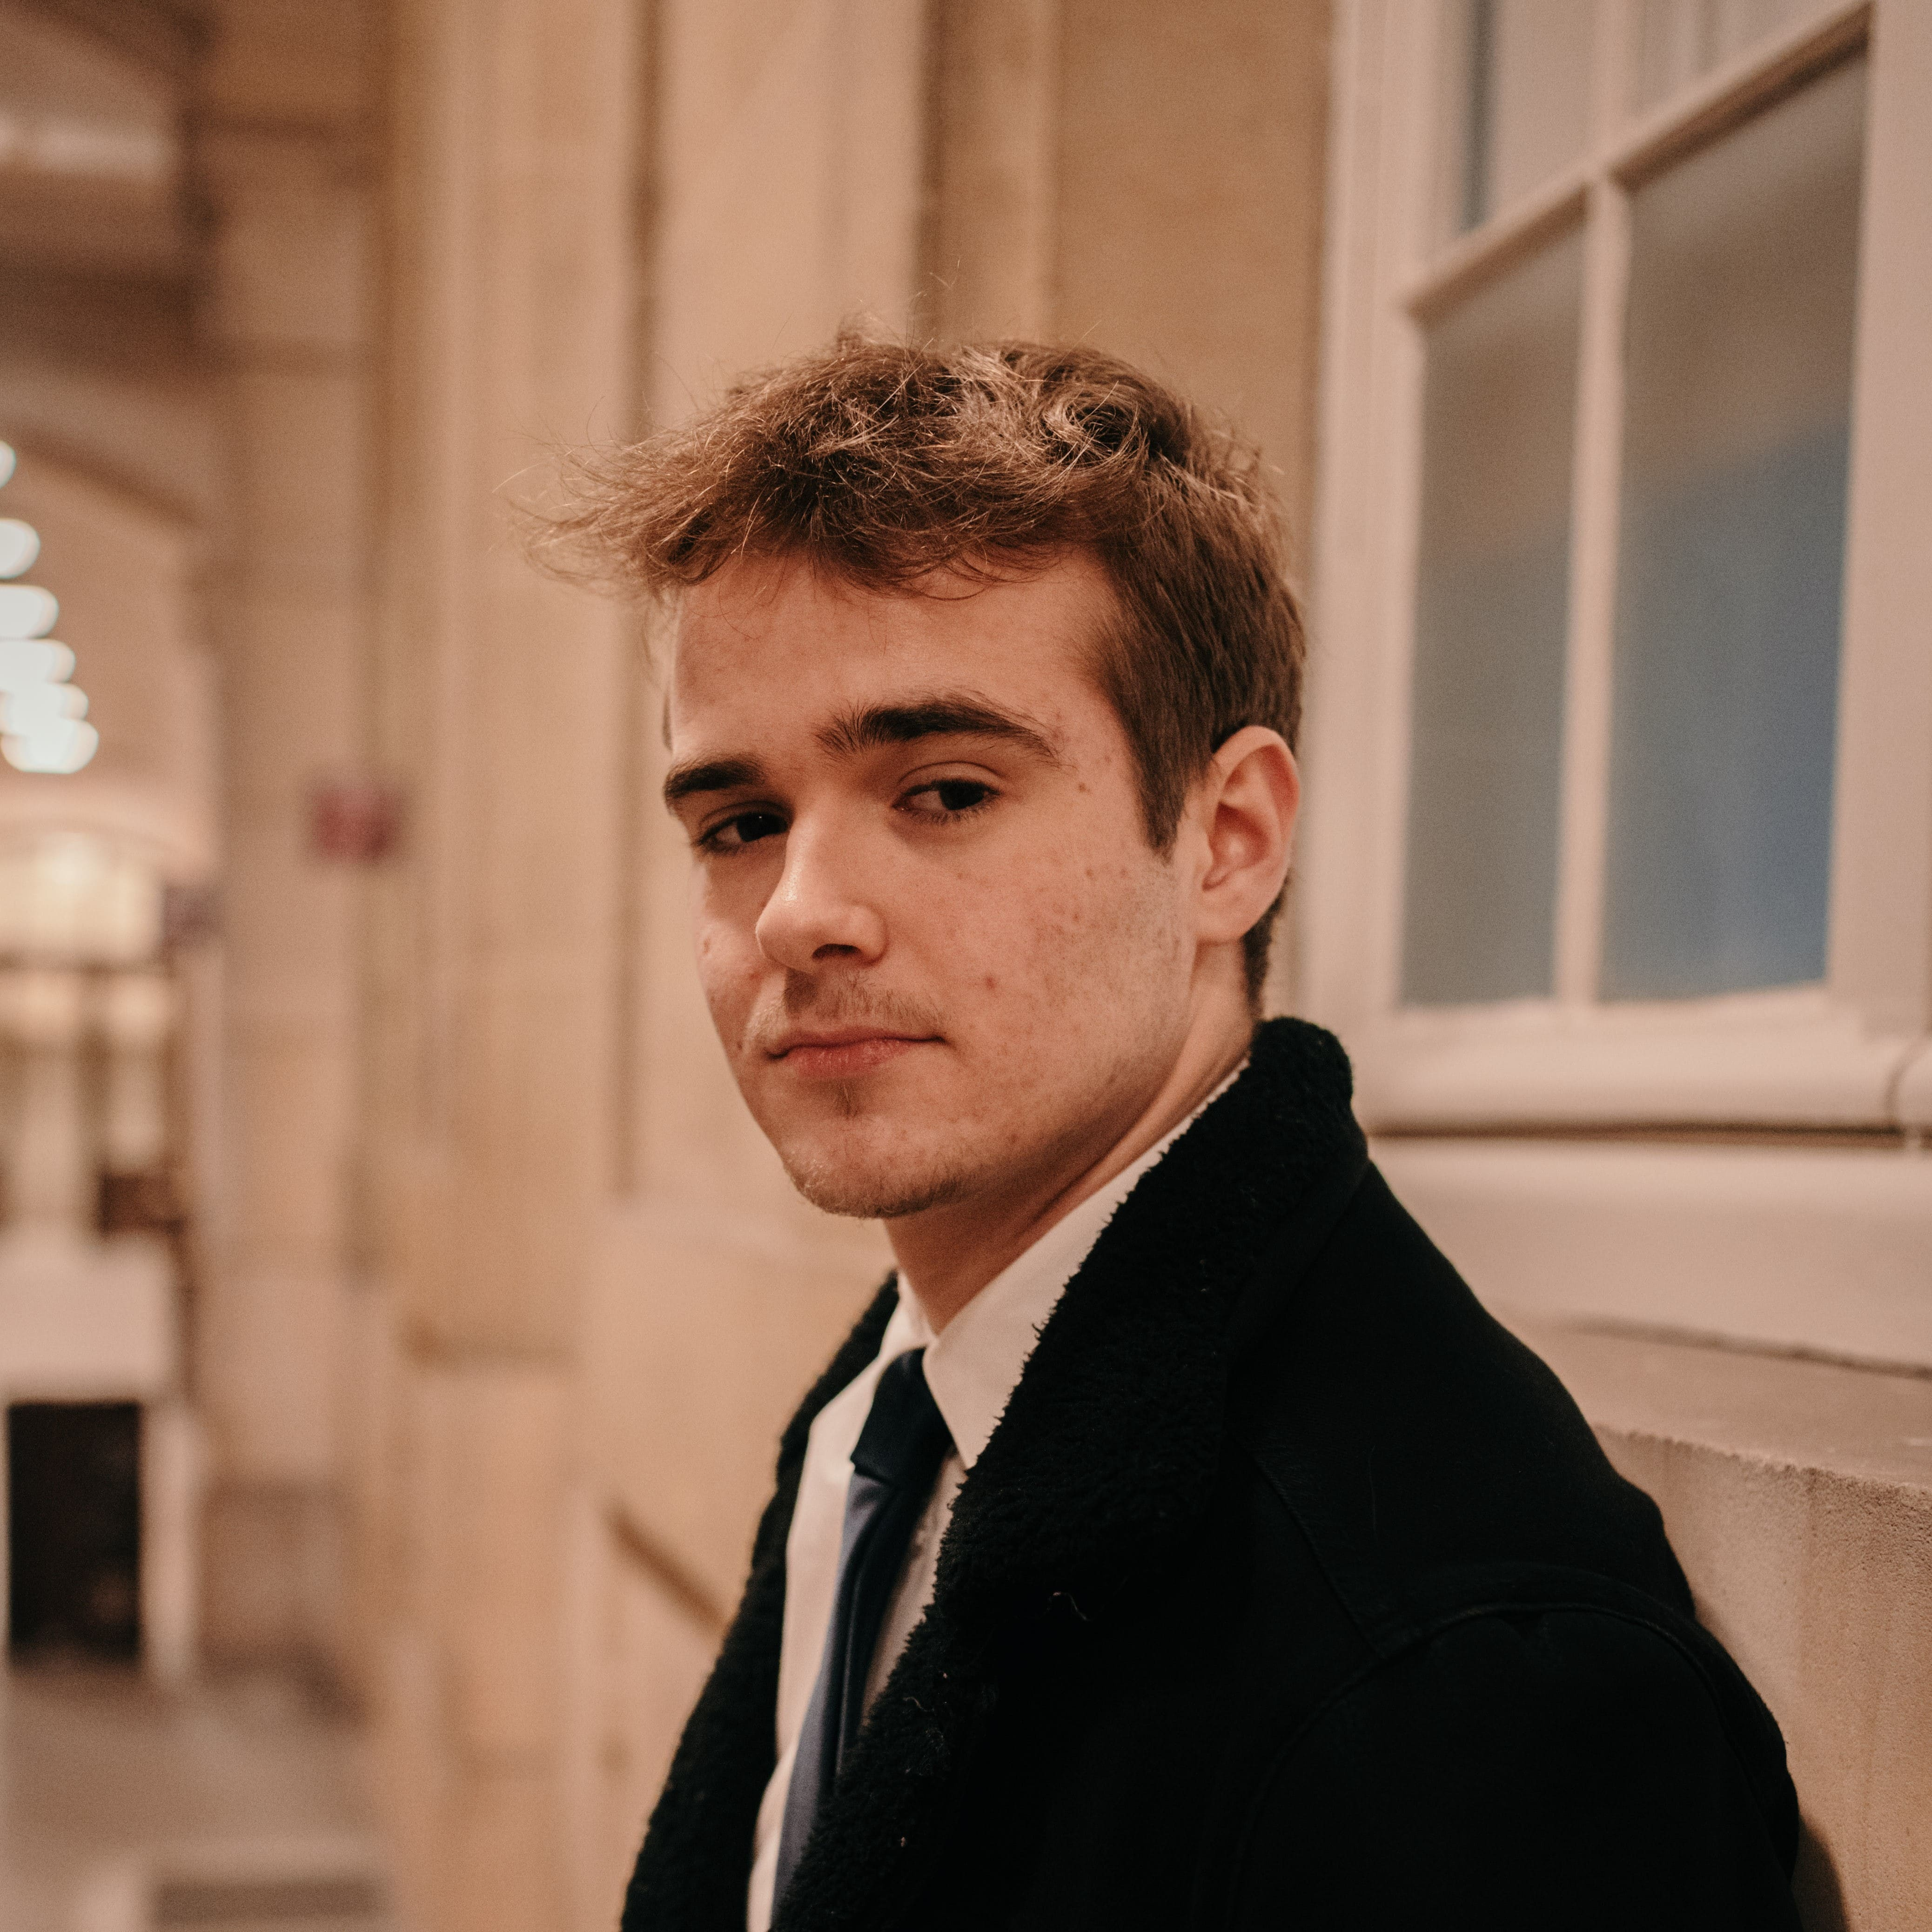
\includegraphics[width=4.5cm]{./photo.jpg}};
        \end{tikzpicture}
    \end{center}
    
    \section*{\sectionicon{\faEnvelope} Contacts}
    \small
    \faPhone\ (+33) 6 56 75 39 83 \\
    \faAt\ contact@ewenrdo.fr \\
    \faMapMarker\ Saint-Gratien, 95210 \\
    \faGlobe\ \href{https://www.ewenrdo.fr}{www.ewenrdo.fr}
    
    \section*{\sectionicon{\faUser} Résumé}
    \footnotesize Étudiant en double licence Maths-Info. Développeur web éco-conçu et responsable, j'allie rigueur mathématique et conception de plateformes logicielles performantes.
    
    \section*{\sectionicon{\faRocket} Compétences}
    \footnotesize
    \textbf{Langages \& Dev :} OCaml, Java, C \\
    \textbf{Web :} React, NestJS, Node.js \\
    \textbf{Outils :} Git, GitHub, VS Code, Linux (UNIX) \\
    \textbf{Maths :} Algèbre, analyse, probabilités
    
    \section*{\sectionicon{\faLanguage} Langues}
    \footnotesize
    FRANÇAIS \hfill \color{iconcolor}\textbf{Natif}\color{black} \\
    ANGLAIS \hfill \color{iconcolor}\textbf{B2 / C1 (Oral)}\color{black}
    
    \section*{\sectionicon{\faCertificate} Certifications}
    \footnotesize
    \textbf{Cambridge English} \\
    B2, C1 oral \hfill \textit{10/2024} \\
    \textbf{Permis B} \hfill \textit{01/2024}
    
    \section*{\sectionicon{\faBriefcase} Engagements}
    \footnotesize\textbf{Notre-Dame de Paris} \hfill 2025 -- 2026 \\
    \textit{Bénévole d'accueil \& médiation}\\
    
    \textbf{Pépite Creaj IDF} \hfill 2024 -- 2025 \\
    \textit{Étudiant-entrepreneur}
\end{minipage}
\hfill
\begin{minipage}[t]{0.65\textwidth}
    % Aligned with the top of the left column
    \vspace{0pt}
    {\Huge \textbf{Ewen Rodrigues de Oliveira}} \\
    
    \vspace{0.3cm}
    \begin{tcolorbox}[colback=titlebg, colframe=titlebg, arc=5pt, left=6pt, right=6pt, top=3pt, bottom=4pt, boxrule=0pt, halign=center, valign=center, width=8.5cm, nobeforeafter]
    \large \textbf{\textsc{\color{iconcolor} ÉTUDIANT MATHS - INFO}}
    \end{tcolorbox}
    
    \vspace{0.5cm}
    \section*{\sectionicon{\faBriefcase} EXPÉRIENCE}
    
    \textbf{Wybz.fr} \hfill 02/2023 -- 11/2025 \\
    \textit{Fondateur \& Développeur Full Stack}
    \begin{itemize}[leftmargin=1em, label=\textbullet]
        \item Création et développement de sites web responsables, éco-conçus, rapides et accessibles.
        \item Développement et maintenance de solutions logicielles et d'écosystèmes web (SaaS).
        \item Pilotage de projets de la conception à la mise en production en autonomie.
    \end{itemize}
    
    \textbf{Lycée Polyvalent Gustave Monod} \hfill 06/2025 \\
    \textit{Stagiaire enseignement (Observation pédagogique)}
    \begin{itemize}[leftmargin=1em, label=\textbullet]
        \item Immersion auprès d'enseignants agrégés de mathématiques dans le secondaire.
        \item Suivi de la démarche pédagogique, préparation de séances et accompagnement des élèves.
    \end{itemize}
    
    \section*{\sectionicon{\faGraduationCap} ÉDUCATION}
    \textbf{Université Paris Cité (Paris Diderot)} \hfill 2024 -- 2027 \\
    \textit{Double licence Mathématiques fondamentales et appliquées / Informatique fondamentale} \\
    \textminus{ Cours avancés, rigueur logique, structures discrètes et programmation.}
    
    \vspace{0.2cm}
    \textbf{Lycée Gustave Monod} \hfill 2024 \\
    \textit{Baccalauréat général -- Mention Très Bien (Section européenne Anglais)}

    \section*{\sectionicon{\faFlask} PROJETS}
    Retrouvez tous mes projets en détail sur mon site web : \href{https://www.ewenrdo.fr/projects}{www.ewenrdo.fr}. Sans exhaustivité, voici quelques projets marquants :
    \begin{itemize}[leftmargin=1em, label=\textbullet]
        \item Création d'éco-systèmes web responsables et performants
        \item Assistant personnel digital pour la gestion du quotidien (connecté aux API de Renault, Proton, Paris Cité, La Poste, etc.).
        \item Jeux vidéos dans le cadre de projets universitaires (Java x Swing).
        \item Rédaction de contenus mathématiques et informatiques pour la distribution aux autres étudiants (exercices, cours, etc.).
    \end{itemize}
\end{minipage}

\end{document}